\section{Aperçu de l'application réalisée}
\label{sec:apercu_application}

Cette section présente ce qu’on voit dans l’application après avoir développé les pages principales. L’idée est de donner une première image de l’interface et des fonctionnalités, sans entrer dans le code.

\subsection{Tableau de bord}
\label{subsec:dashboard}

Le tableau de bord est la page d’accueil après connexion. On y trouve un résumé rapide des courriers et des notifications, pour savoir tout de suite si quelque chose demande une action.

\begin{figure}[H]
    \centering
    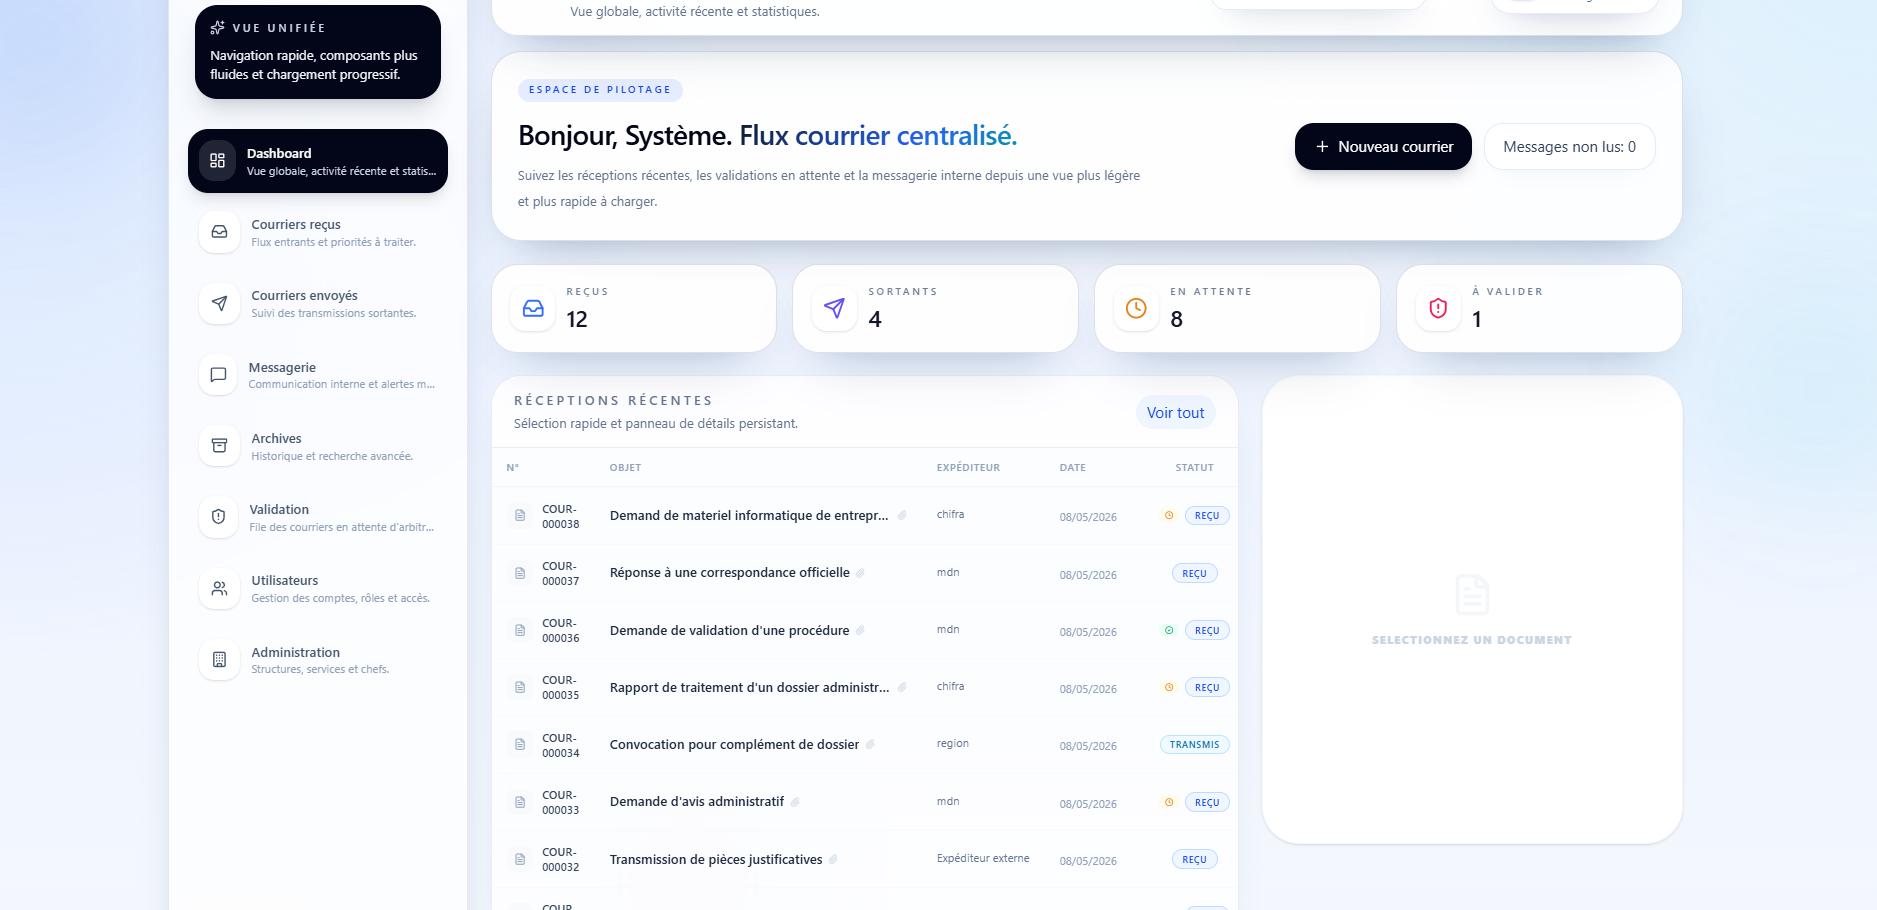
\includegraphics[width=0.92\textwidth,height=0.46\textheight,keepaspectratio]{images/app/dashboard.png}
    \caption{Vue du tableau de bord}
    \label{fig:dashboard_preview}
\end{figure}

\subsection{Gestion des courriers reçus}
\label{subsec:courriers_recus}

Cette partie du site regroupe tous les courriers entrants traités par l’application. L’utilisateur peut consulter la liste, filtrer et aller vers un courrier précis.

\begin{figure}[H]
    \centering
    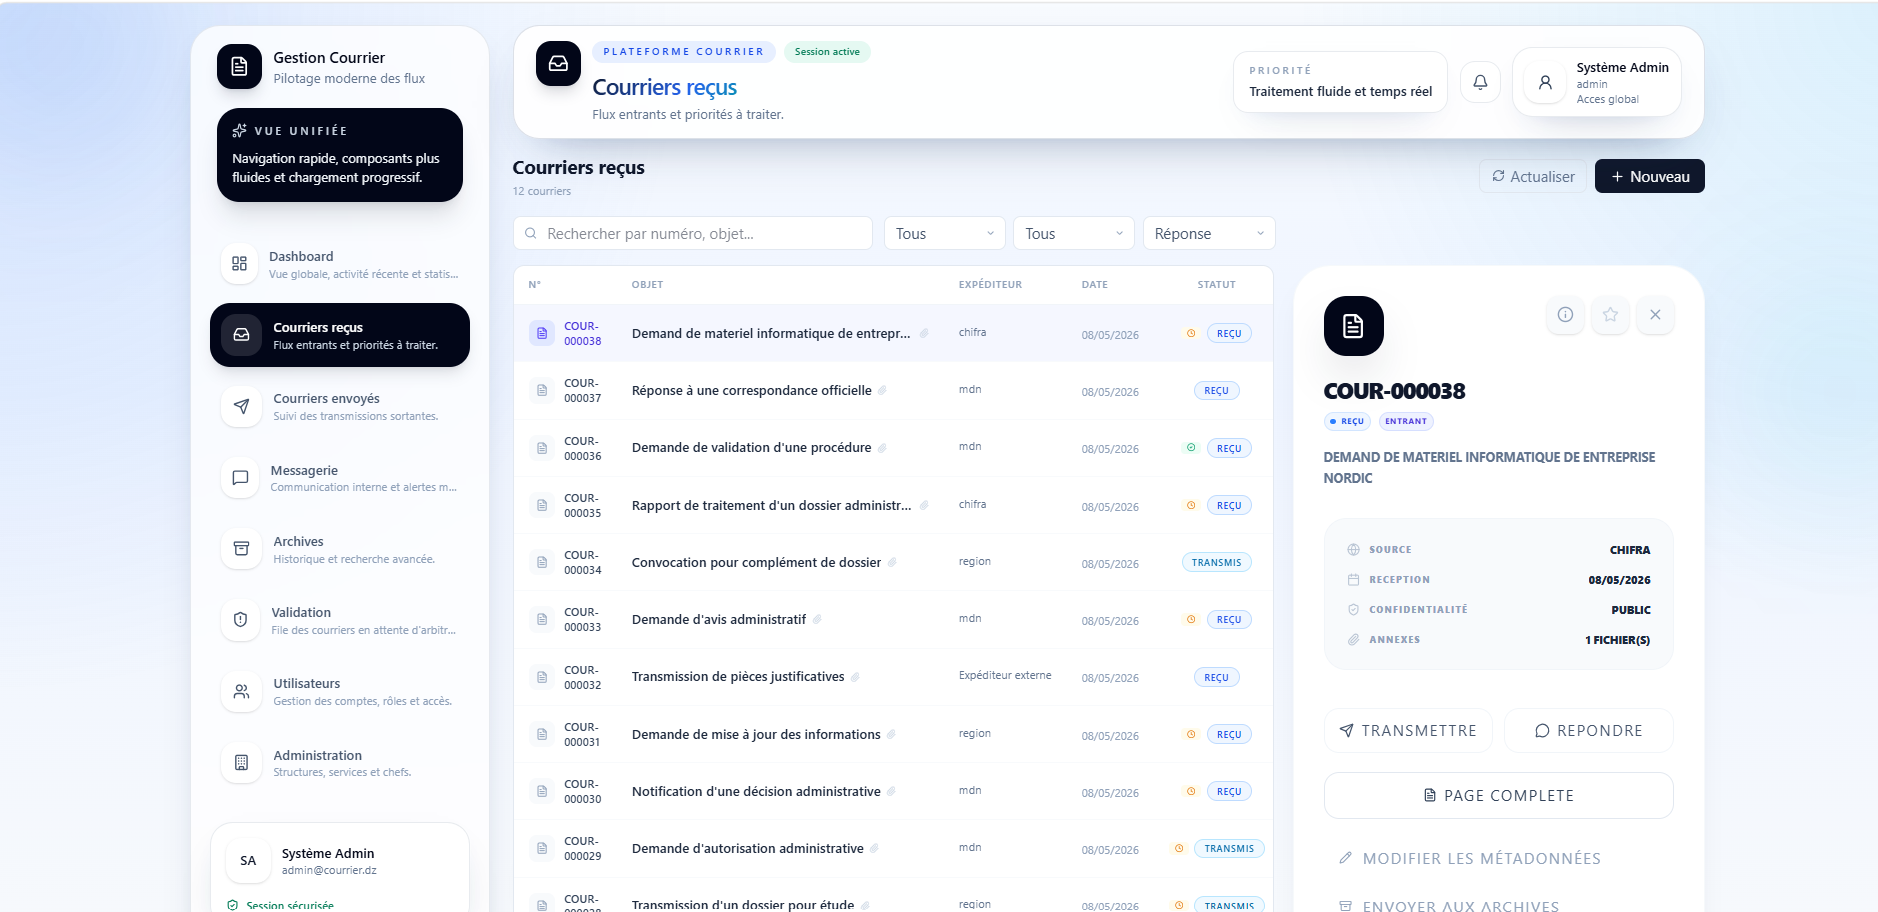
\includegraphics[width=0.92\textwidth,height=0.46\textheight,keepaspectratio]{images/app/courier_recu.png}
    \caption{Liste des courriers reçus}
    \label{fig:courriers_recus_list}
\end{figure}

\subsubsection{Création d’un nouveau courrier reçu}
\label{subsubsec:creation_courrier_recu}

La création d’un courrier reçu se fait avec un formulaire qui accepte l’objet, le service destinataire, la date et les pièces jointes. C’est la base pour entrer les documents qui arrivent dans l’organisation.

\begin{figure}[H]
    \centering
    \begin{minipage}{0.49\textwidth}
        \centering
        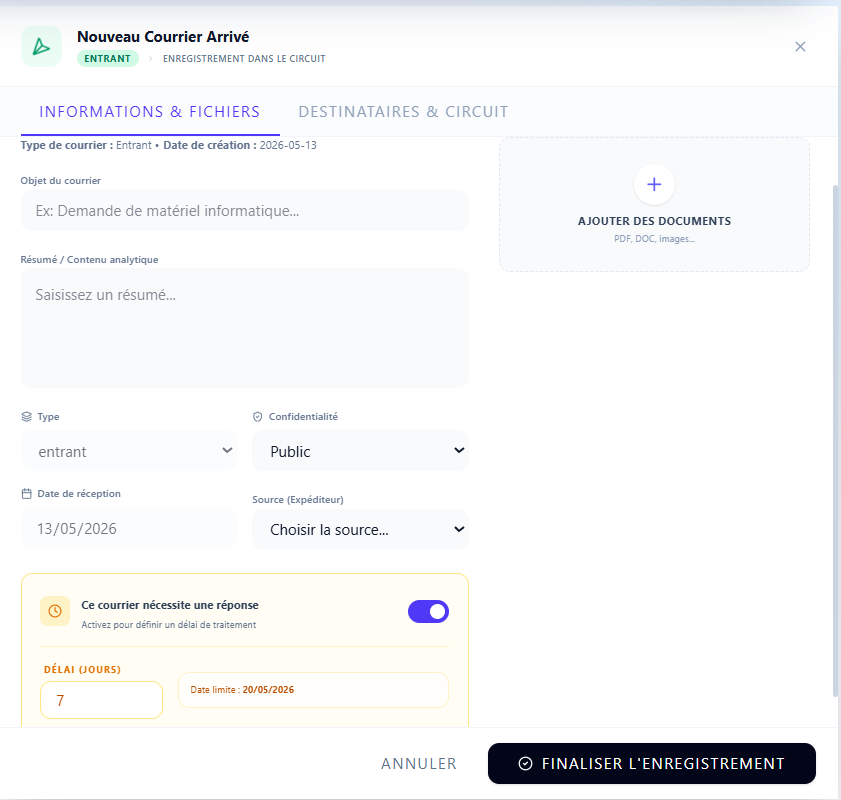
\includegraphics[width=\linewidth,height=0.36\textheight,keepaspectratio]{images/app/courier_recu_crre1.png}
    \end{minipage}
    \hfill
    \begin{minipage}{0.49\textwidth}
        \centering
        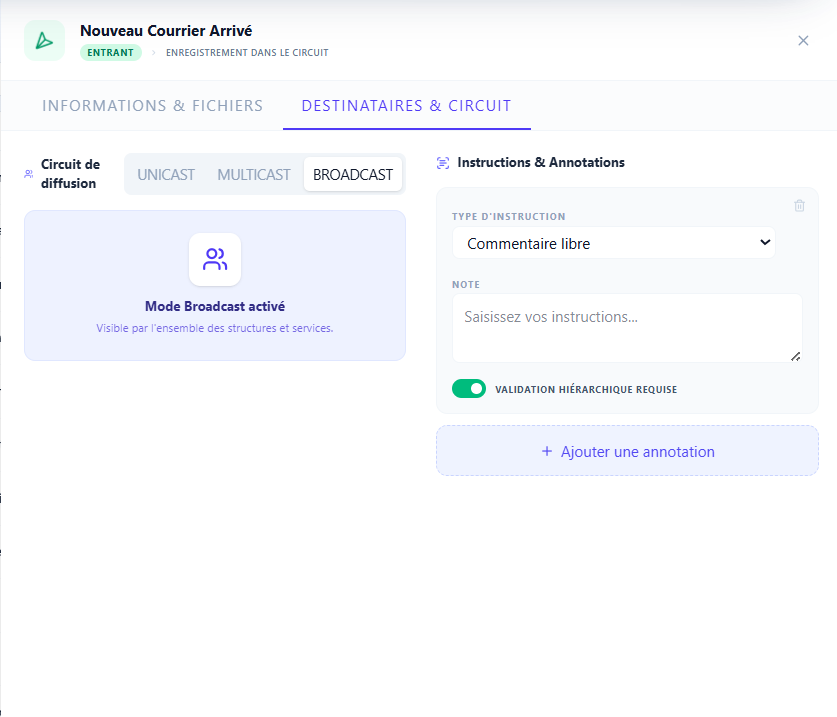
\includegraphics[width=\linewidth,height=0.36\textheight,keepaspectratio]{images/app/courier_recu_crr2.png}
    \end{minipage}
    \caption{Formulaire de création d’un courrier reçu}
    \label{fig:creation_courrier_recu}
\end{figure}

\subsubsection{Transmission d’un courrier}
\label{subsubsec:transmission_courrier}

Quand il faut transférer un courrier vers un autre service ou responsable, la transmission permet d’avancer le dossier. L’interface propose un bouton de transmission et un suivi d’état simple.

\begin{figure}[H]
    \centering
    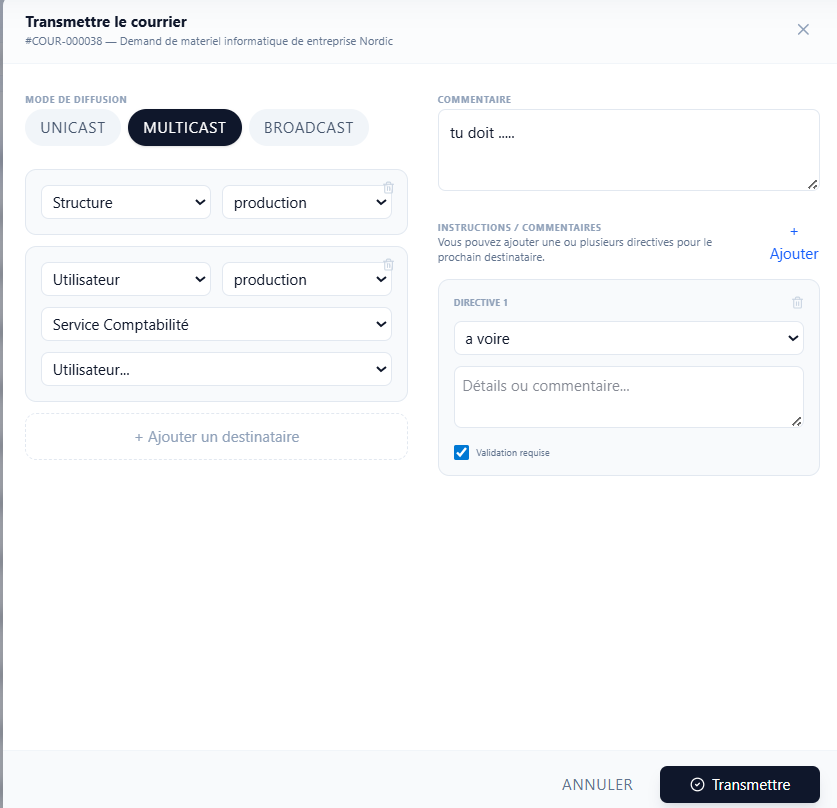
\includegraphics[width=0.90\textwidth,height=0.44\textheight,keepaspectratio]{images/app/trans.png}
    \caption{Écran de transmission d’un courrier}
    \label{fig:transmission_courrier}
\end{figure}

\subsubsection{Réponse à un courrier}
\label{subsubsec:reponse_courrier}

La réponse à un courrier s’effectue depuis le détail du courrier reçu, avec un formulaire pré-rempli et des destinataires suggérés selon le workflow.

\begin{figure}[H]
    \centering
    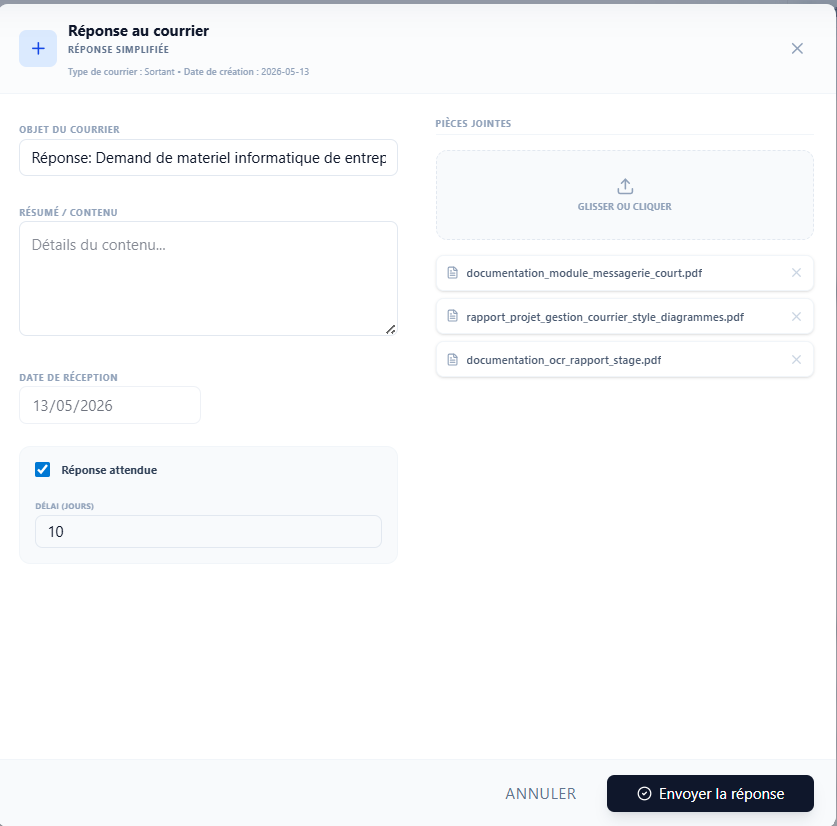
\includegraphics[width=0.90\textwidth,height=0.3\textheight,keepaspectratio]{images/app/respo_cor.png}
    \caption{Interface de réponse à un courrier}
    \label{fig:reponse_courrier}
\end{figure}

\subsubsection{Archivage d’un courrier}
\label{subsubsec:archivage_courrier}

L’archivage permet de ranger un courrier hors du flux actif, tout en le gardant accessible pour consultation future. Le système retire le courrier de la vue principale sans le supprimer.

\begin{figure}[H]
    \centering
    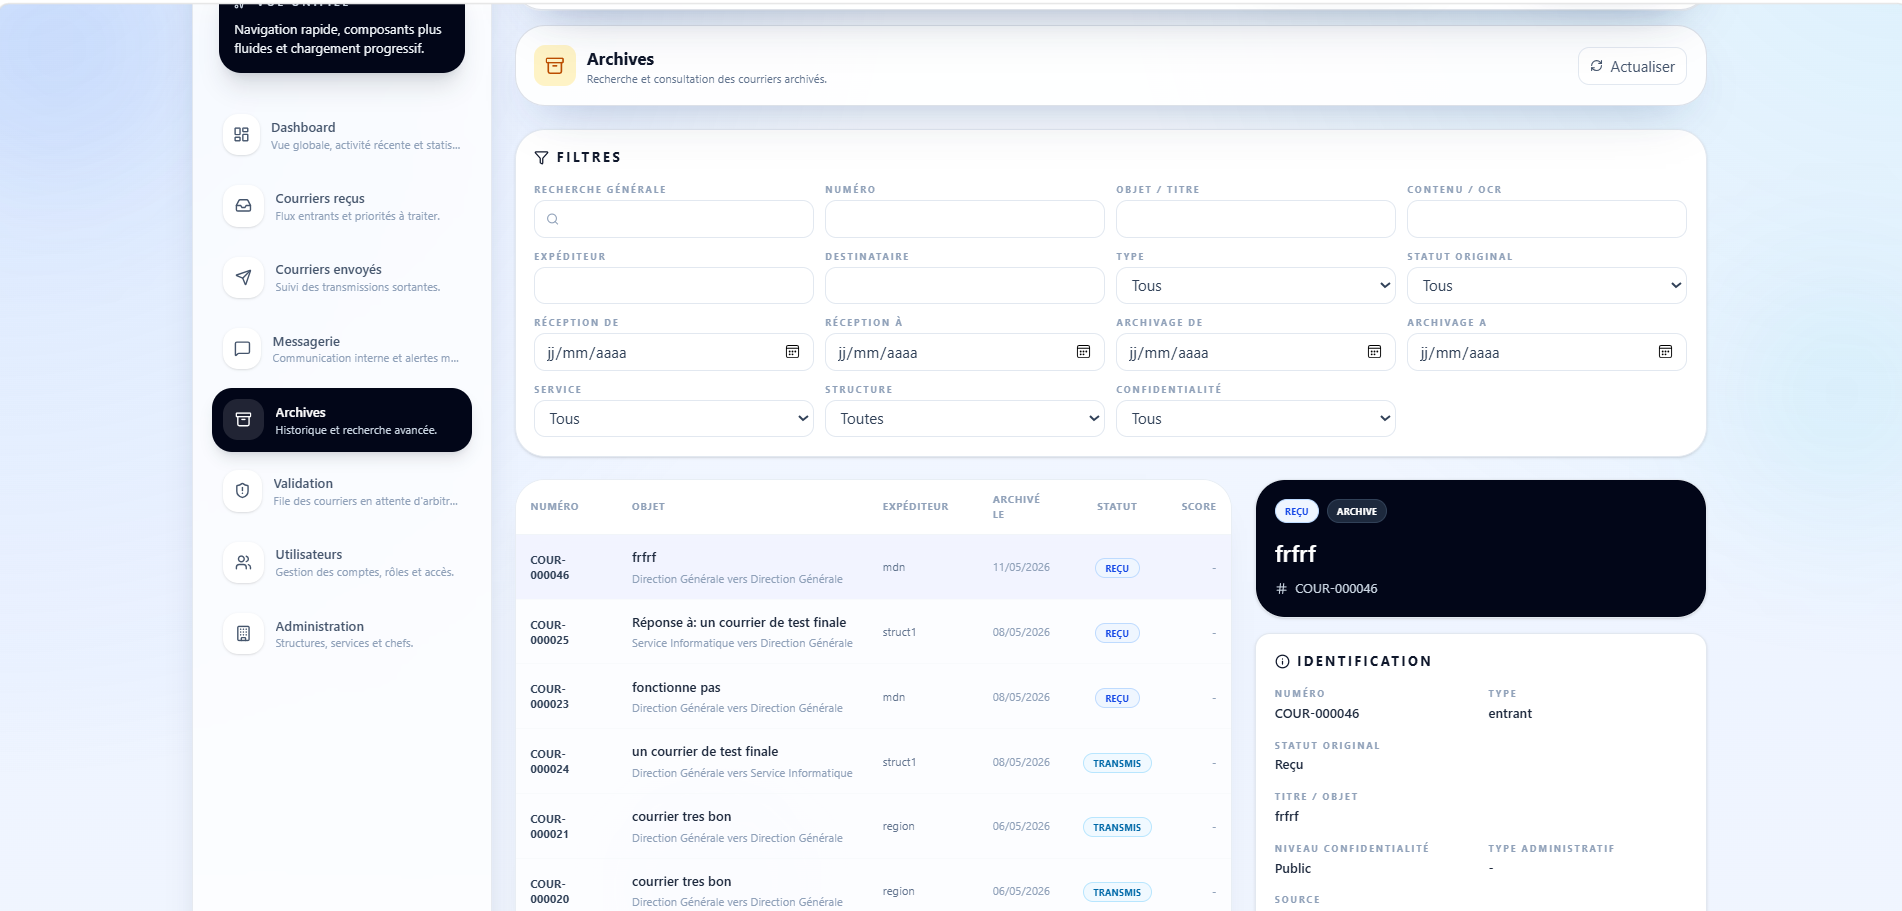
\includegraphics[width=0.90\textwidth,height=0.44\textheight,keepaspectratio]{images/app/archive.png}
    \caption{Archivage d’un courrier}
    \label{fig:archivage_courrier}
\end{figure}


\subsection{Gestion des courriers envoyés}
\label{subsec:courriers_envoyes}

Cette section liste les courriers sortants. Elle montre les envois déjà effectués, les brouillons et les éléments en attente de validation.

\begin{figure}[H]
    \centering
    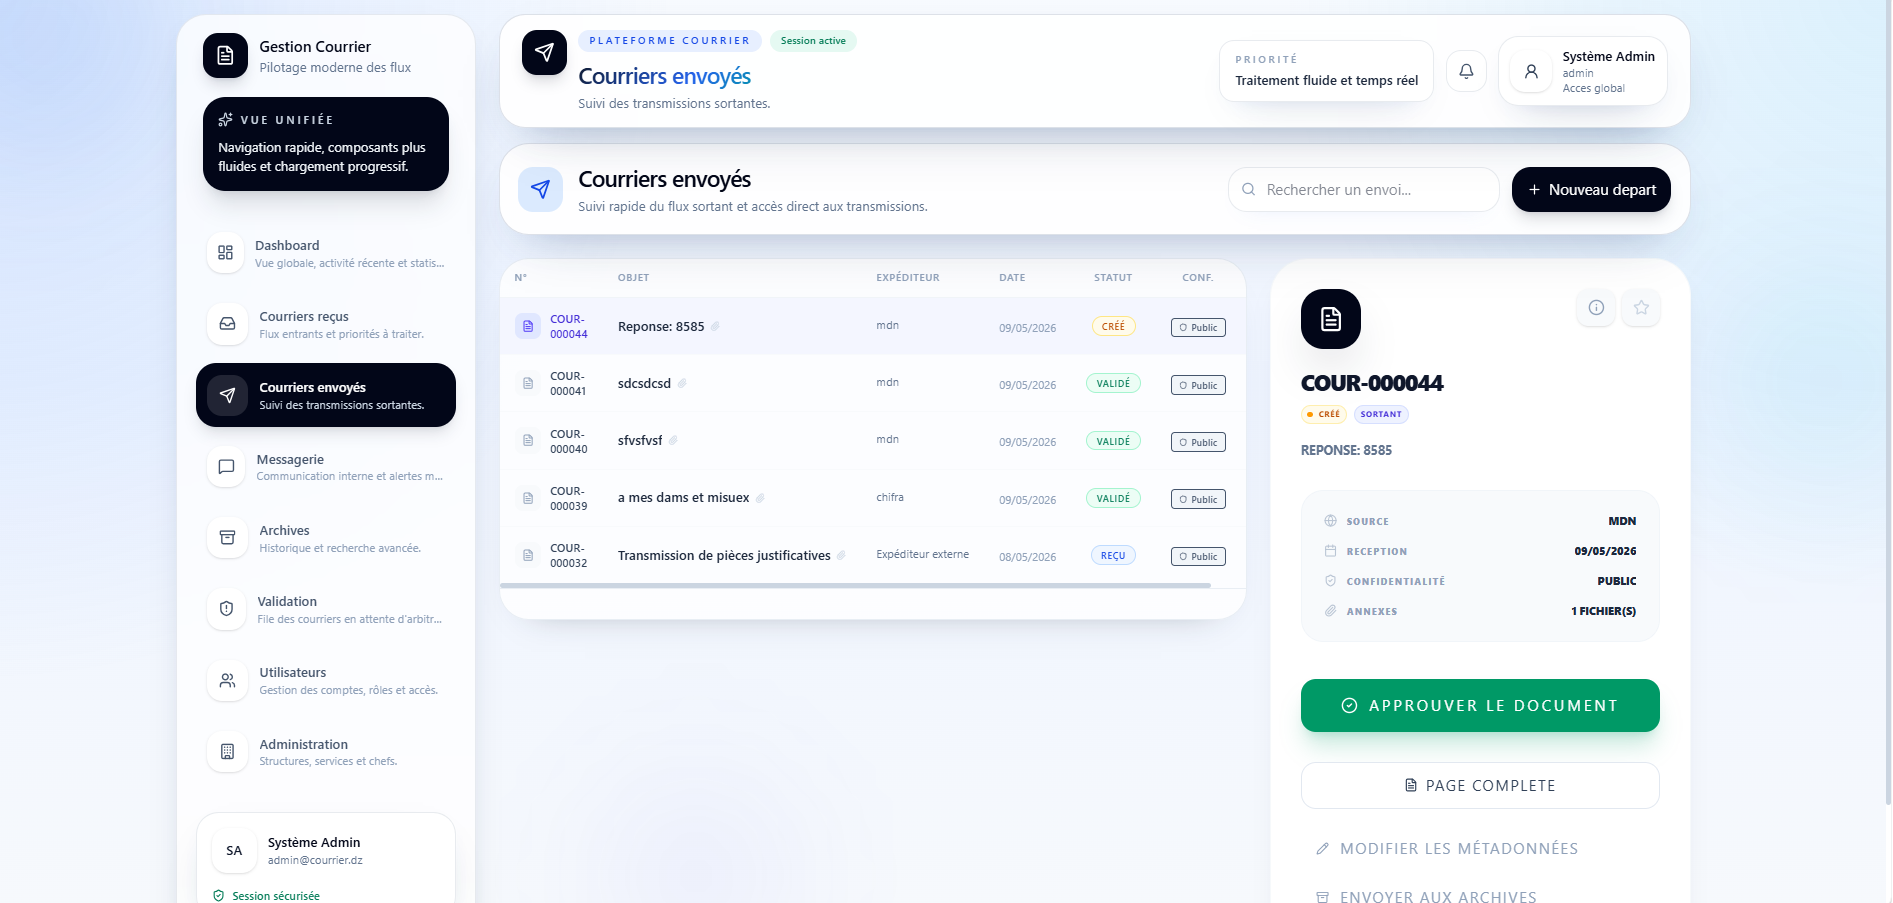
\includegraphics[width=0.92\textwidth,height=0.40\textheight,keepaspectratio]{images/app/courrier_env.png}
    \caption{Liste des courriers envoyés}
    \label{fig:courriers_envoyes}
\end{figure}

\subsubsection{Création d’un nouveau courrier envoyé}
\label{subsubsec:creation_courrier_envoye}

Le formulaire d’envoi permet de rédiger un courrier sortant, de choisir la confidentialité et les destinataires, puis de l’enregistrer ou de le soumettre.

\begin{figure}[H]
    \centering
    \begin{minipage}{0.49\textwidth}
        \centering
        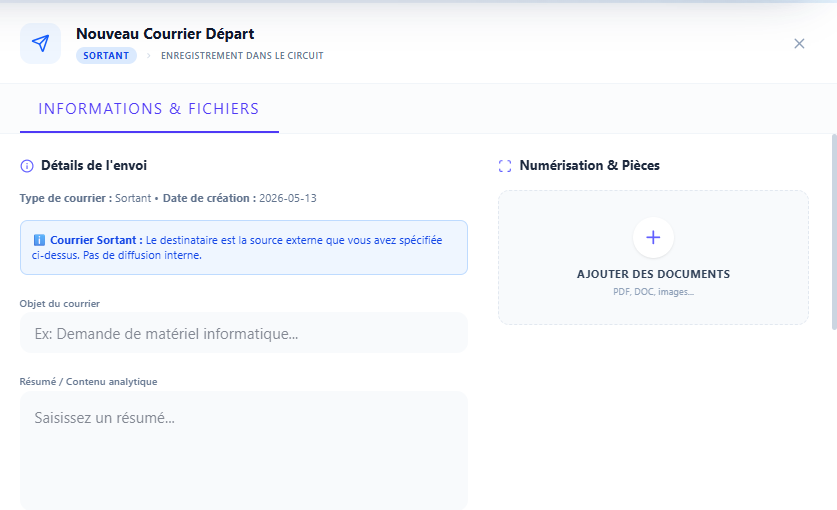
\includegraphics[width=\linewidth,height=0.36\textheight,keepaspectratio]{images/app/Courier_envoye_create.png}
    \end{minipage}
    \hfill
    \begin{minipage}{0.49\textwidth}
        \centering
        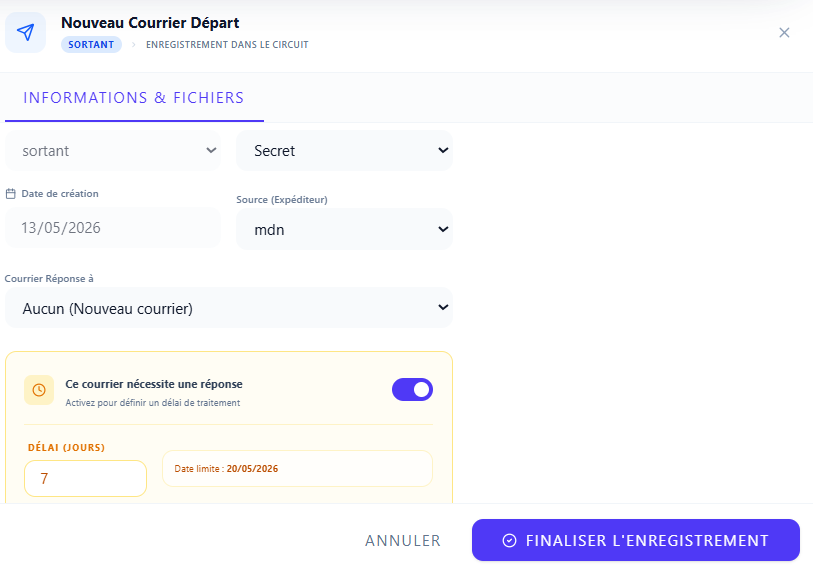
\includegraphics[width=\linewidth,height=0.36\textheight,keepaspectratio]{images/app/coureur_env_crea2.png}
    \end{minipage}
    \caption{Formulaire de création d’un courrier envoyé}
    \label{fig:creation_courrier_envoye}
\end{figure}

\subsection{Messagerie interne}
\label{subsec:messagerie_interne}

La messagerie interne sert à communiquer rapidement entre utilisateurs quand un courrier ne suffit pas. Elle permet d’envoyer et de recevoir des messages privés.

\begin{figure}[H]
    \centering
    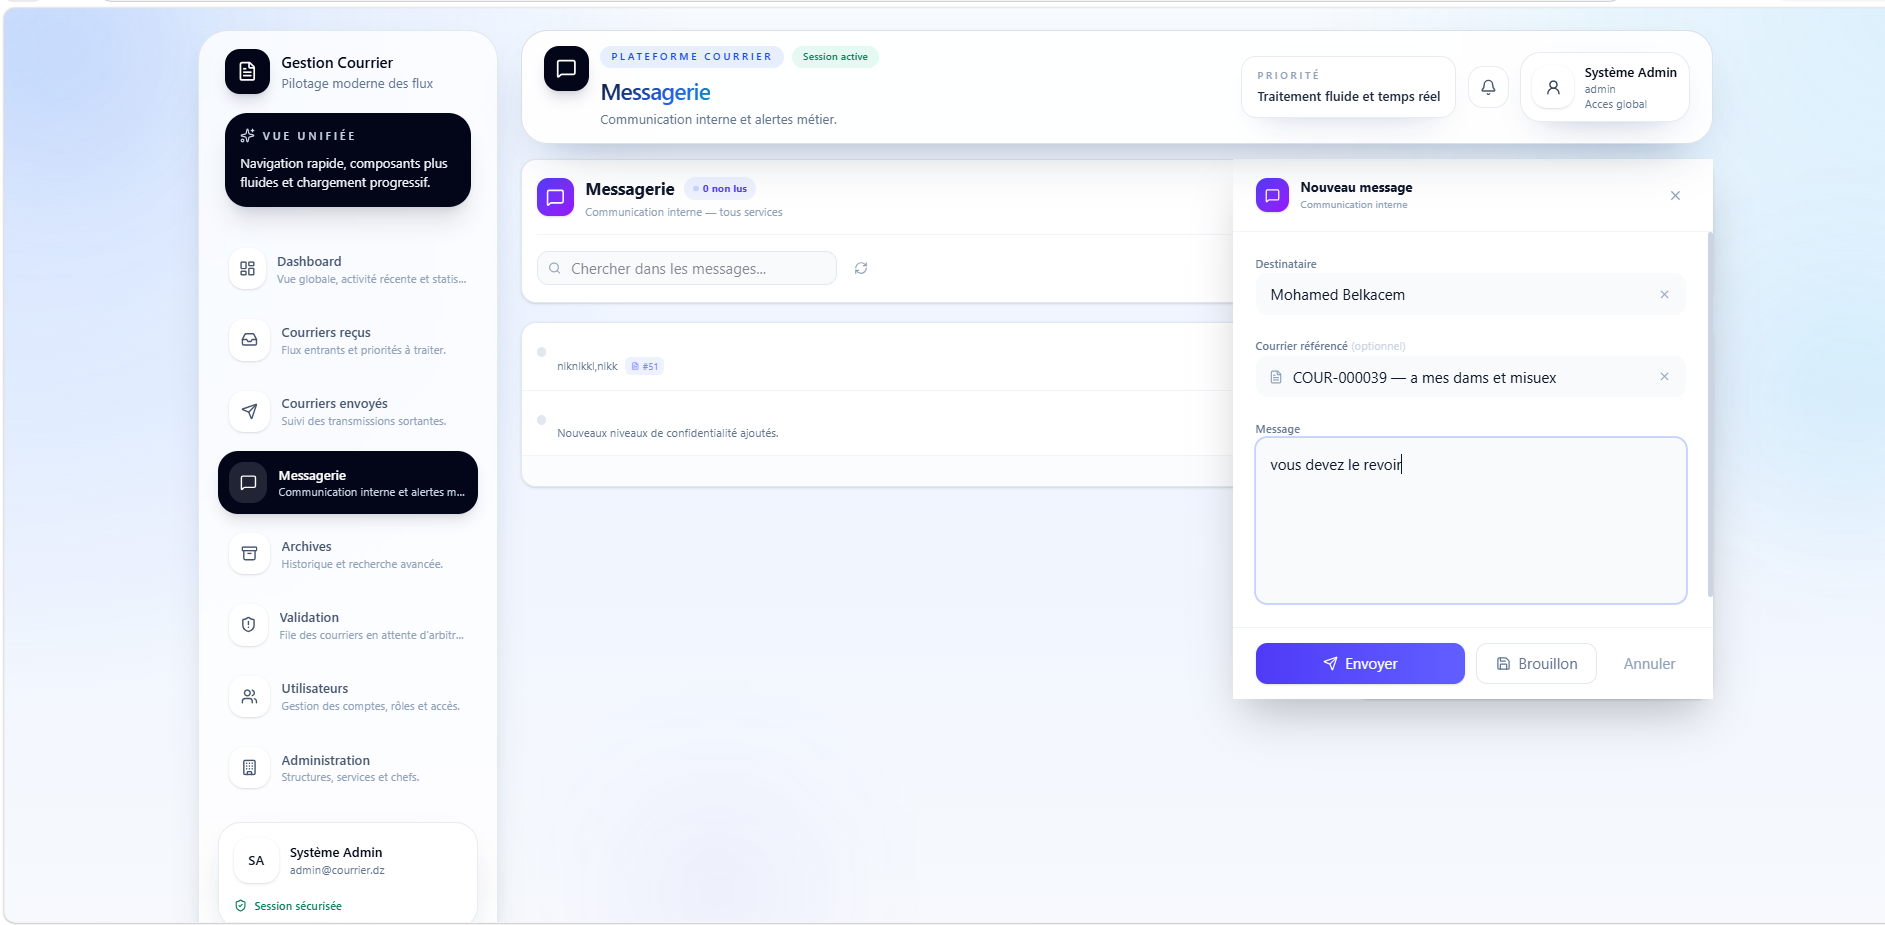
\includegraphics[width=0.90\textwidth,height=0.44\textheight,keepaspectratio]{images/app/msg_+create.png}
    \caption{Messagerie interne}
    \label{fig:messagerie_interne}
\end{figure}

\subsubsection{Création d’un nouveau message}
\label{subsubsec:creation_message}

L’utilisateur compose son message, choisit un destinataire et peut l’envoyer ou le sauvegarder en brouillon. C’est simple et direct.

\begin{figure}[H]
    \centering
    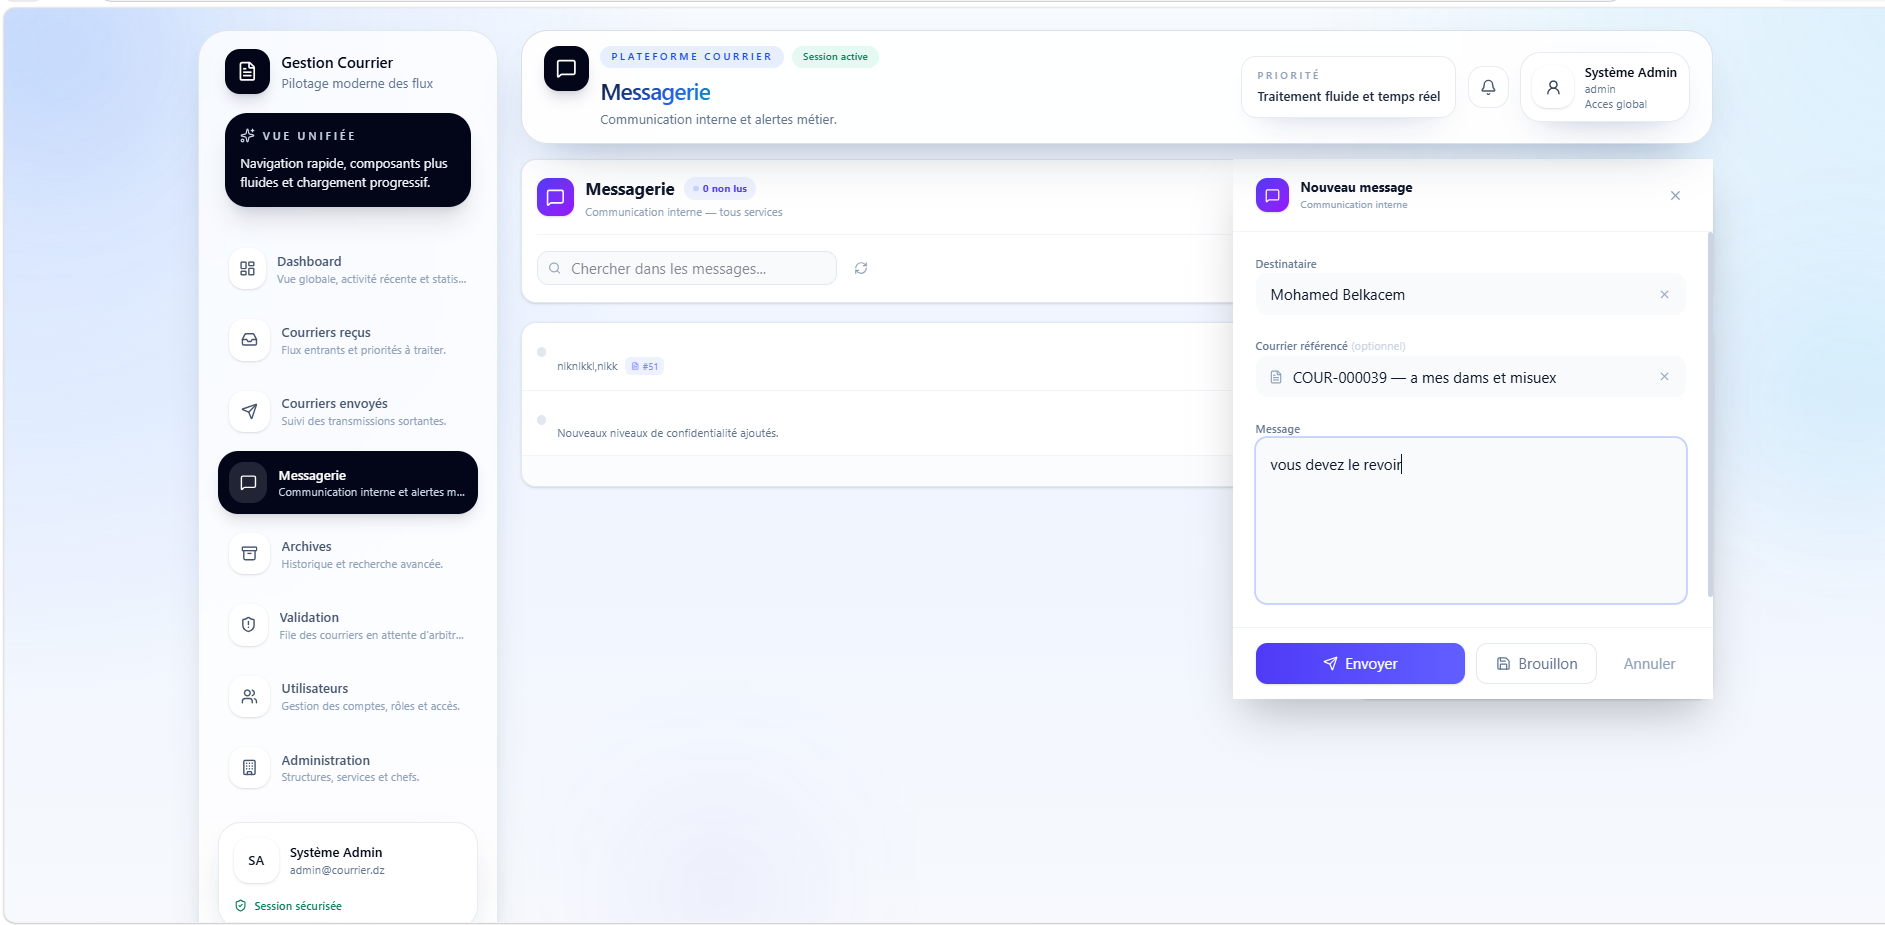
\includegraphics[width=0.90\textwidth,height=0.44\textheight,keepaspectratio]{images/app/msg_+create.png}
    \caption{Création d’un nouveau message}
    \label{fig:creation_message}
\end{figure}

\subsubsection{Consultation des messages}
\label{subsubsec:consultation_messages}

La consultation permet de lire les messages reçus et envoyés, avec le statut lu/non-lu et la possibilité de filtrer par destinataire.

\begin{figure}[H]
    \centering
    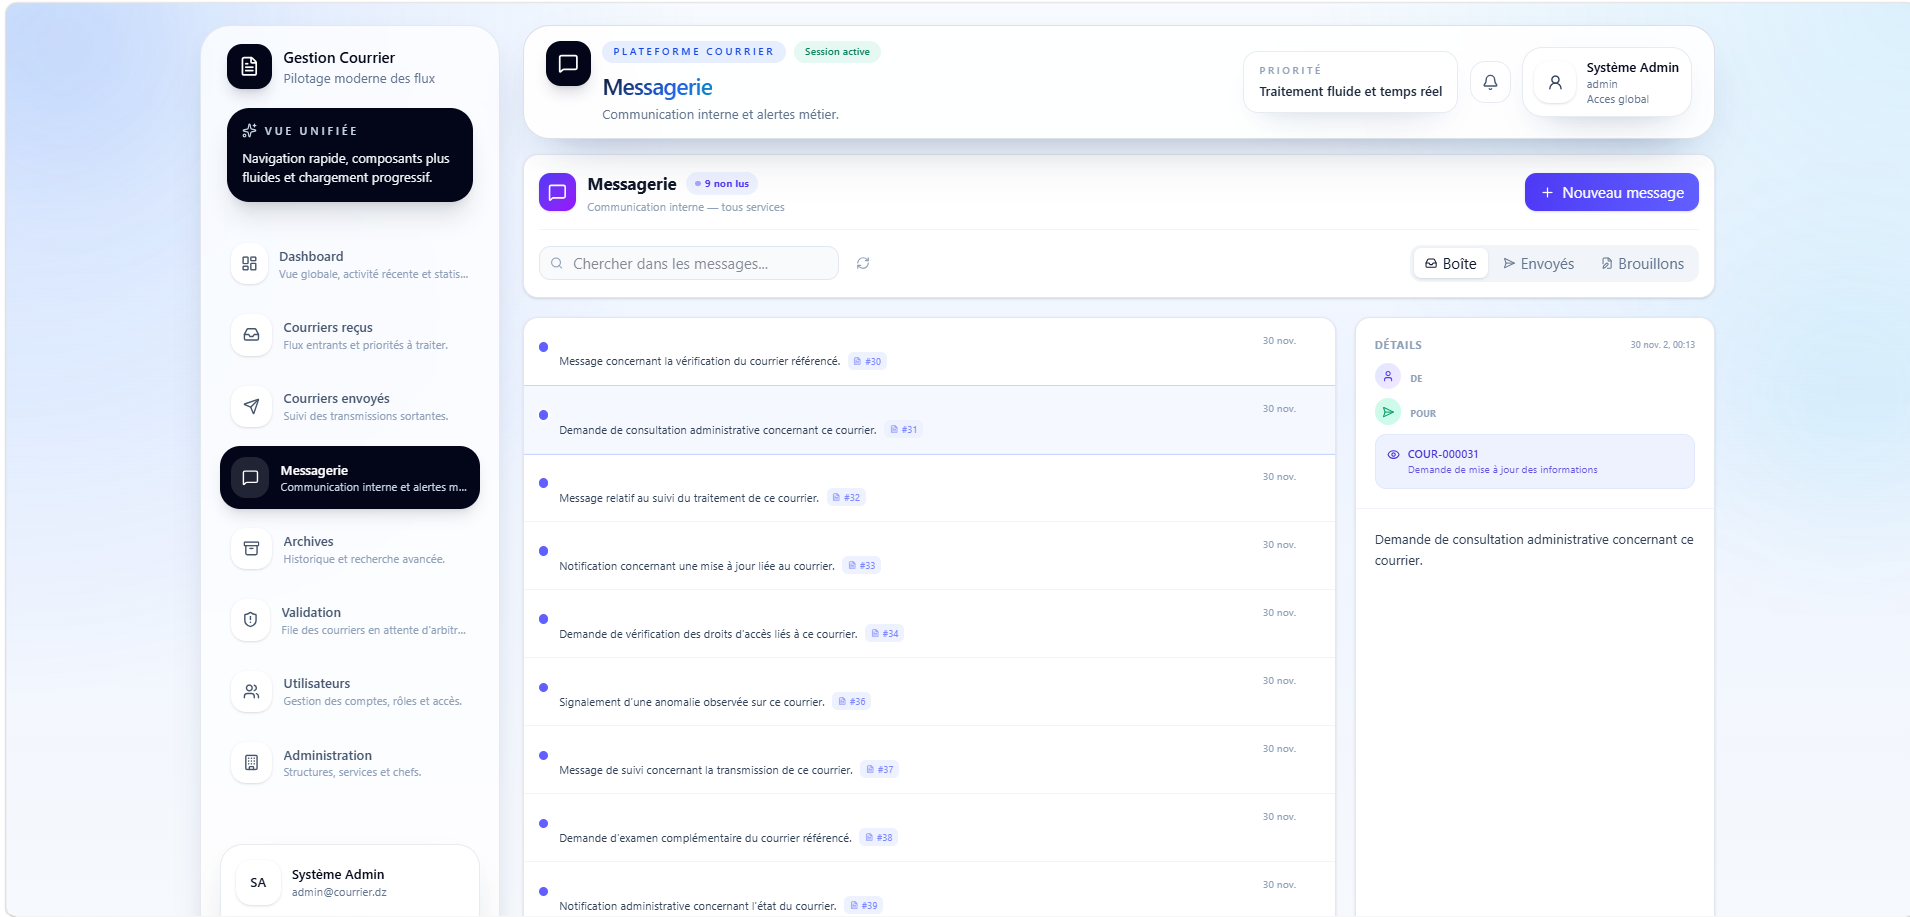
\includegraphics[width=0.90\textwidth,height=0.44\textheight,keepaspectratio]{images/app/cons_im.png}
    \caption{Consultation des messages}
    \label{fig:consultation_messages}
\end{figure}

\subsection{Gestion des archives}
\label{subsec:gestion_archives}

La gestion des archives permet de retrouver un courrier classé par le passé. C’est utile pour garder l’historique sans encombrer les listes actives.

\begin{figure}[H]
    \centering
    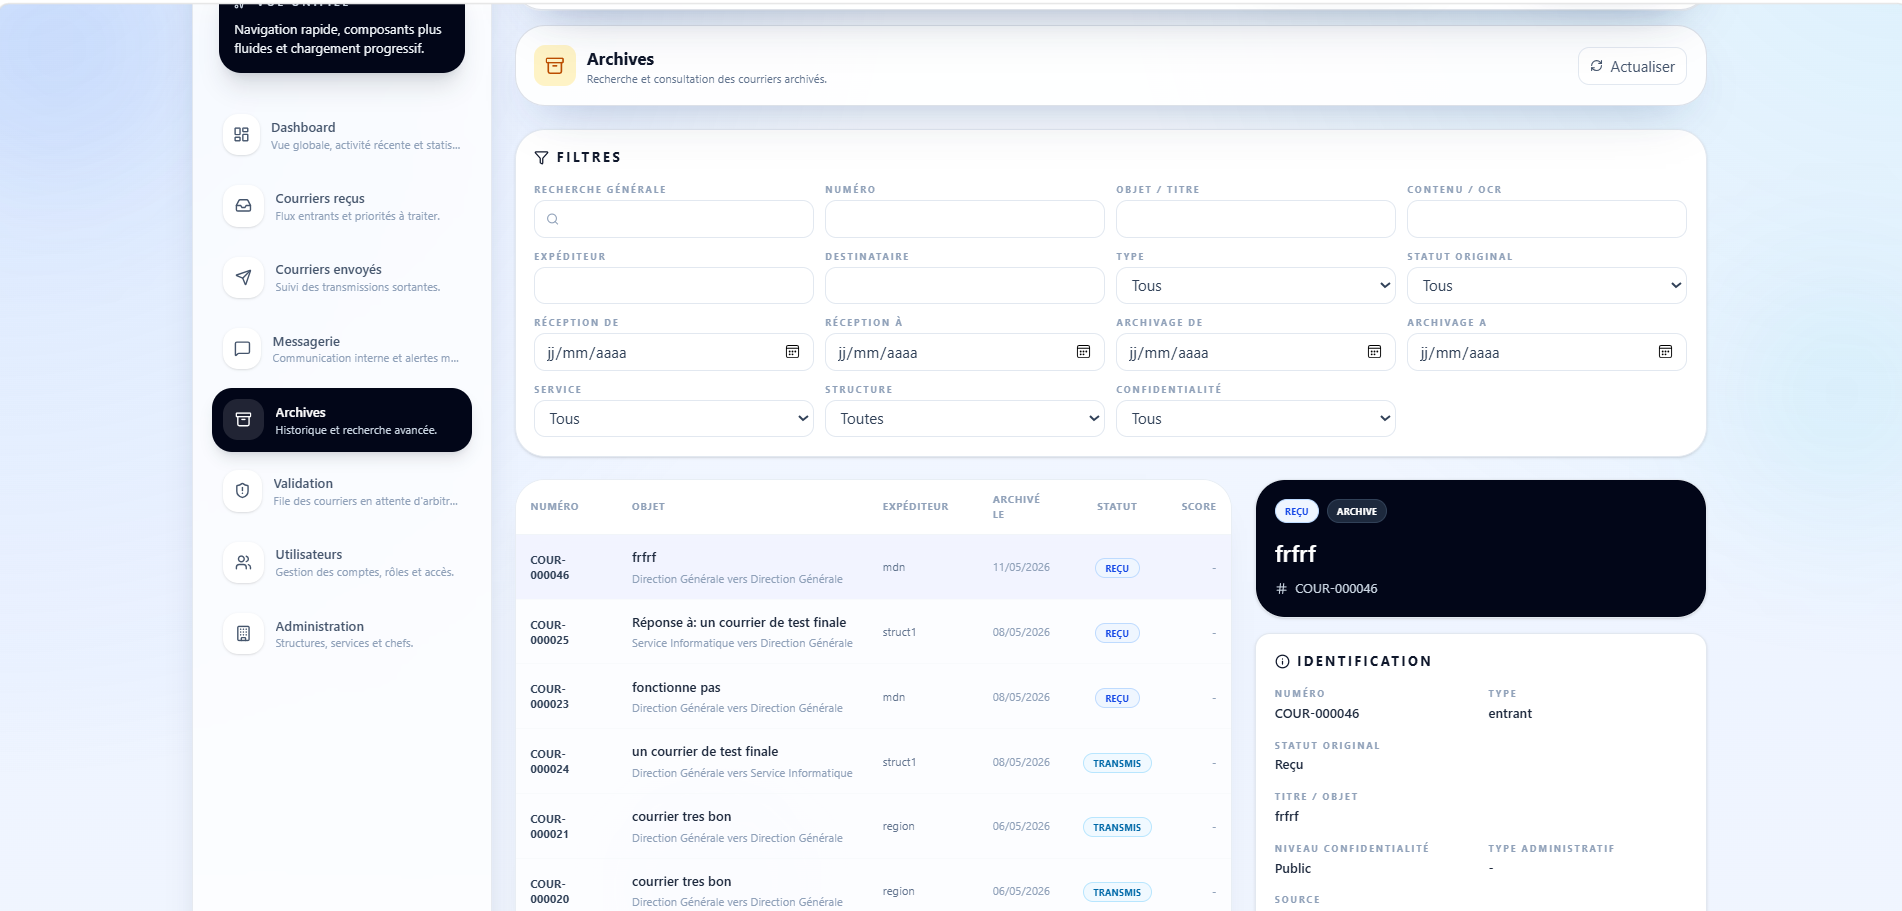
\includegraphics[width=0.90\textwidth,height=0.44\textheight,keepaspectratio]{images/app/archive.png}
    \caption{Vue de la gestion des archives}
    \label{fig:gestion_archives}
\end{figure}

\subsubsection{Recherche et filtrage des courriers archivés}
\label{subsubsec:recherche_filtre_archives}

Le moteur de recherche des archives accepte plusieurs critères : numéro, objet, date ou statut. Cela aide à retrouver rapidement un courrier ancien.

\begin{figure}[H]
    \centering
    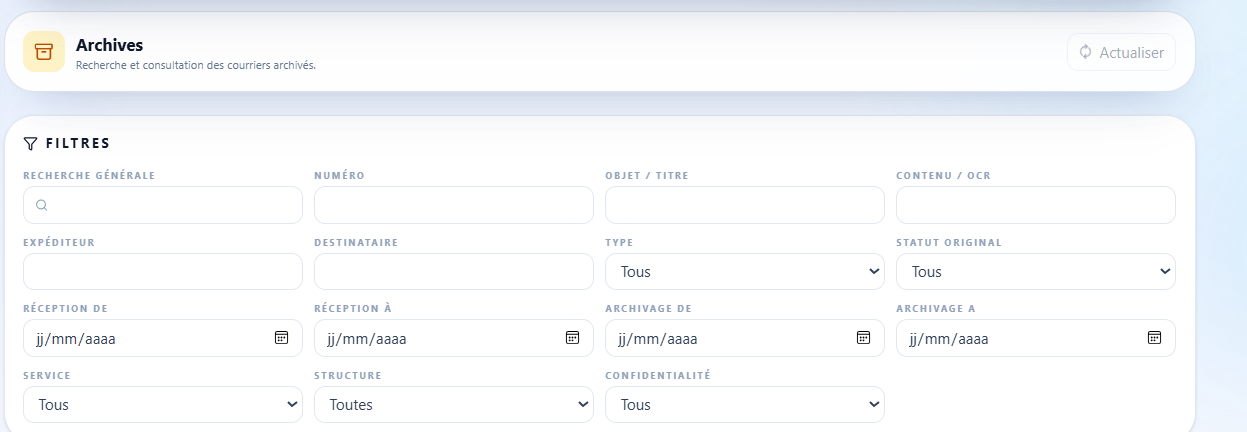
\includegraphics[width=0.90\textwidth,height=0.44\textheight,keepaspectratio]{images/app/filtre.png}
    \caption{Recherche et filtrage des archives}
    \label{fig:recherche_filtre_archives}
\end{figure}


\subsection{Gestion de l’administration}
\label{subsec:gestion_administration}

Cette partie est réservée à l’administrateur. Elle permet d’organiser les entités de l’application, notamment les structures, les services et l’affectation des responsables. Grâce à ces interfaces, l’administration peut préparer l’environnement de travail avant l’utilisation quotidienne du système par les autres profils.
\subsubsection{Gestion des utilisateurs}
\label{subsec:gestion_utilisateurs}

Cette page de gestion est destinée aux administrateurs. Elle affiche les profils utilisateurs, les rôles et les droits, et permet de modifier ou supprimer des comptes.

\begin{figure}[H]
    \centering
    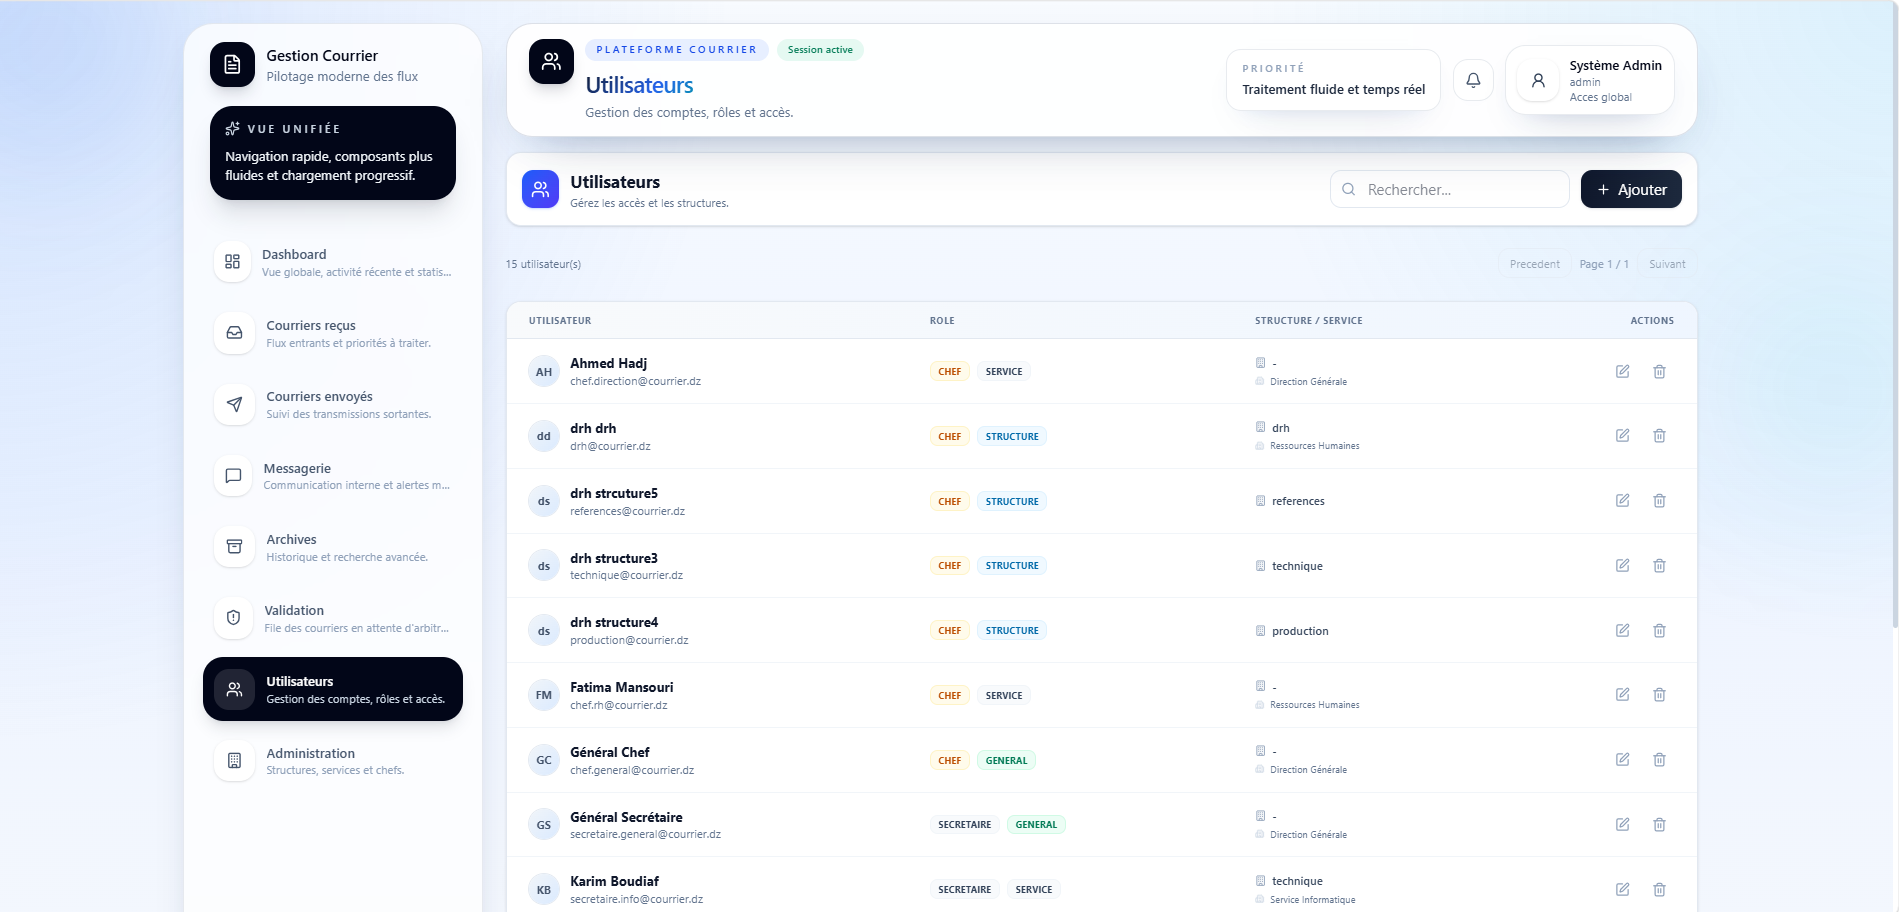
\includegraphics[width=0.90\textwidth,height=0.44\textheight,keepaspectratio]{images/app/users_index.png}
    \caption{Gestion des utilisateurs}
    \label{fig:gestion_utilisateurs}
\end{figure}

\subsubsection{Affichage des structures}
\label{subsubsec:affichage_structures}

L’affichage des structures permet à l’administrateur de consulter les différentes entités organisationnelles enregistrées dans l’application. Cette interface facilite le suivi des structures existantes et prépare les opérations d’ajout, de modification ou de suppression.

\begin{figure}[H]
    \centering
    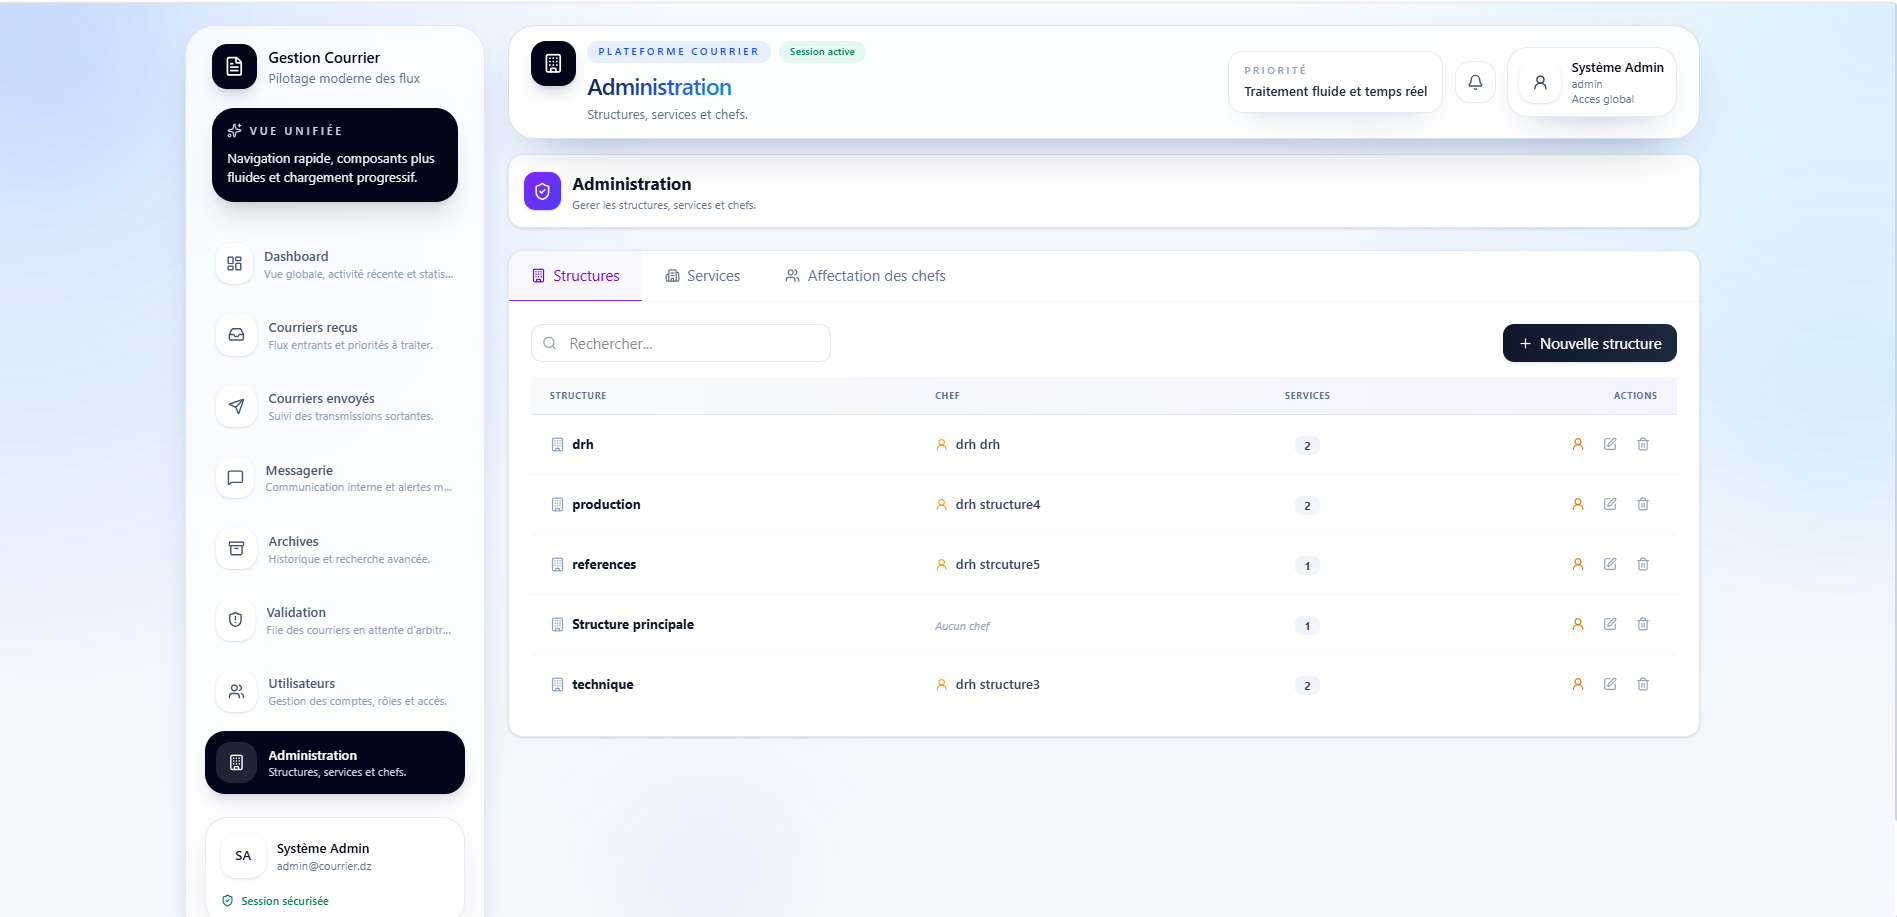
\includegraphics[width=0.92\textwidth,height=0.46\textheight,keepaspectratio]{images/app/adminstrationindex.png}
    \caption{Affichage des structures}
    \label{fig:affichage_structures}
\end{figure}

\subsubsection{Création d’une structure}
\label{subsubsec:creation_structure}

La création d’une structure permet d’ajouter une direction ou une entité organisationnelle dans le système. Cette structure pourra ensuite être utilisée pour rattacher des services et organiser les utilisateurs.

\begin{figure}[H]
    \centering
    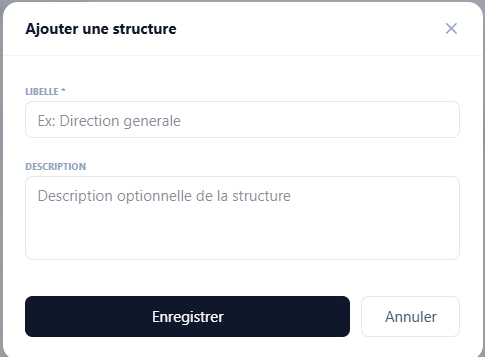
\includegraphics[width=0.88\textwidth,height=0.42\textheight,keepaspectratio]{images/app/struct_crr.png}
    \caption{Création d’une structure}
    \label{fig:creation_structure}
\end{figure}

\subsubsection{Affichage des services}
\label{subsubsec:affichage_services}

L’affichage des services présente la liste des services disponibles dans l’application. Chaque service est rattaché à une structure, ce qui permet de mieux organiser les utilisateurs et les circuits de traitement des courriers.

\begin{figure}[H]
    \centering
    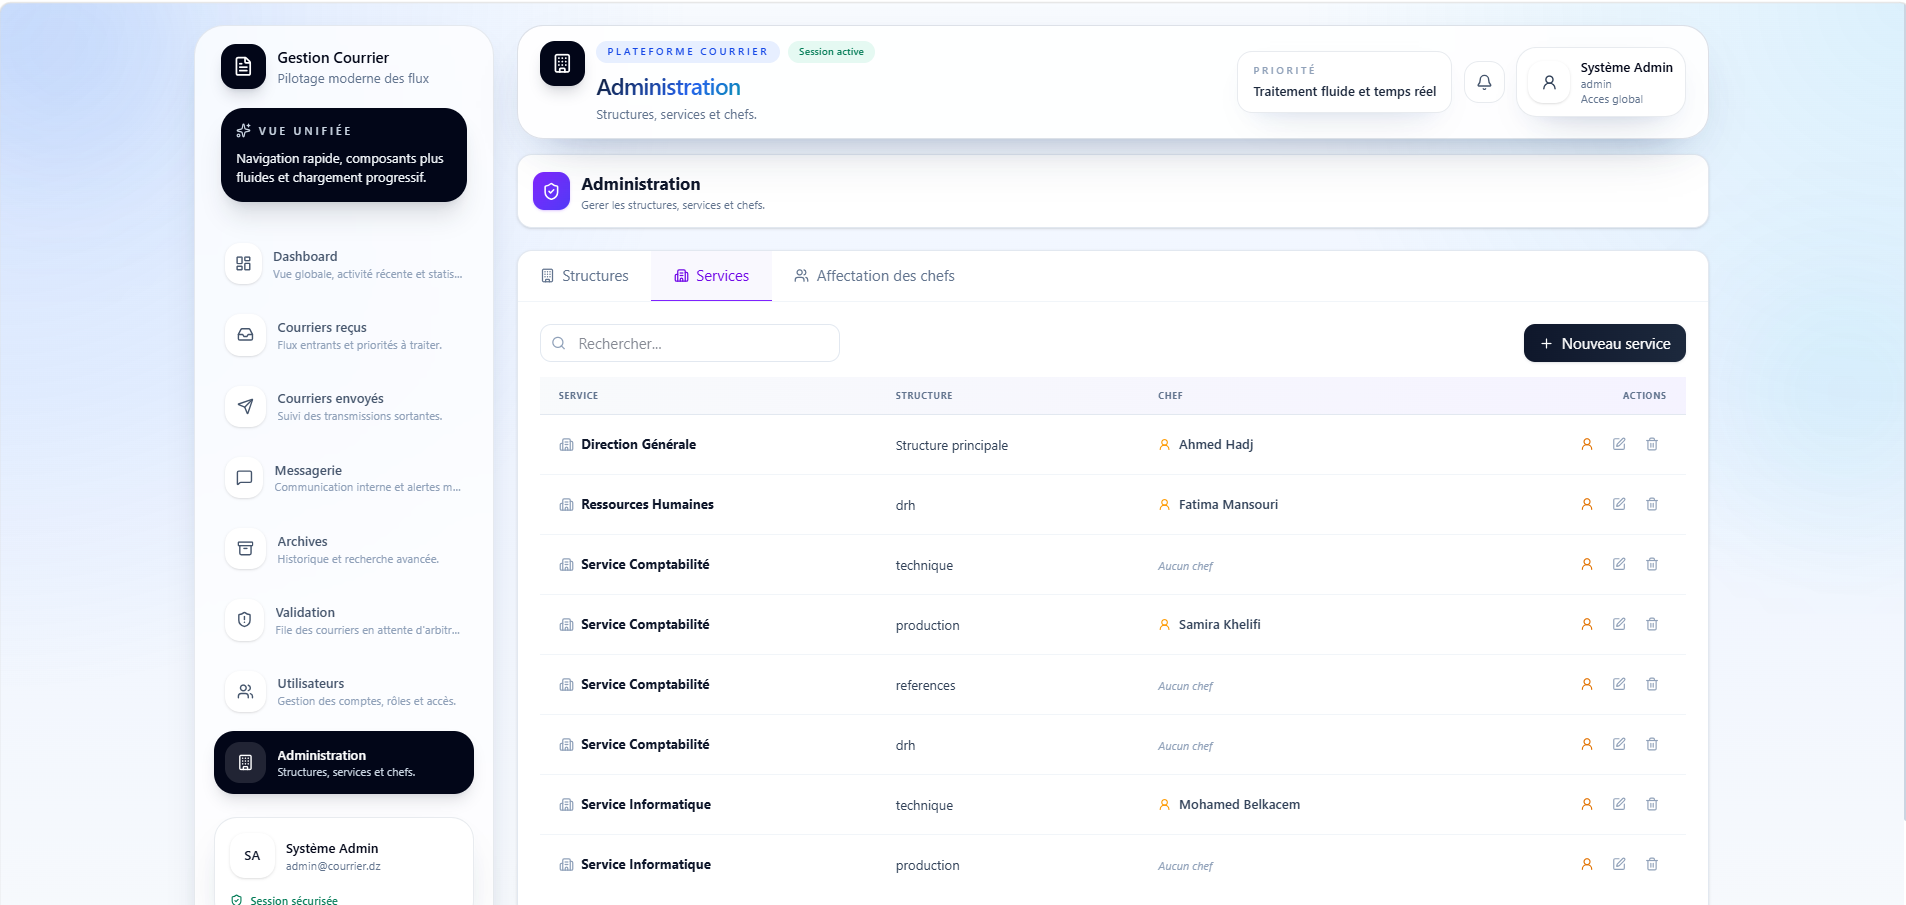
\includegraphics[width=0.92\textwidth,height=0.46\textheight,keepaspectratio]{images/app/services.png}
    \caption{Affichage des services}
    \label{fig:affichage_services}
\end{figure}

\subsubsection{Création d’un service}
\label{subsubsec:creation_service}

La création d’un service permet de définir les différents départements rattachés à une structure. Chaque service peut ensuite être utilisé dans la gestion des courriers, des utilisateurs et des droits d’accès.

\begin{figure}[H]
    \centering
    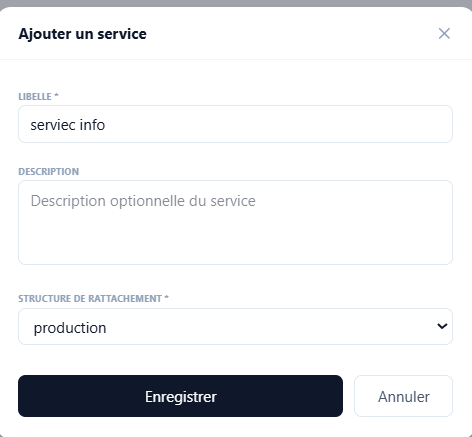
\includegraphics[width=0.88\textwidth,height=0.36\textheight,keepaspectratio]{images/app/services1.png}
    \caption{Création d’un service}
    \label{fig:creation_service}
\end{figure}

\subsubsection{Affectation des responsables}
\label{subsubsec:affectation_responsables}

L’affectation permet d’associer un responsable à une structure ou à un service. Cette étape est importante pour appliquer correctement les règles de validation, de transmission et de consultation des courriers selon le rôle de chaque utilisateur.

\begin{figure}[H]
    \centering
    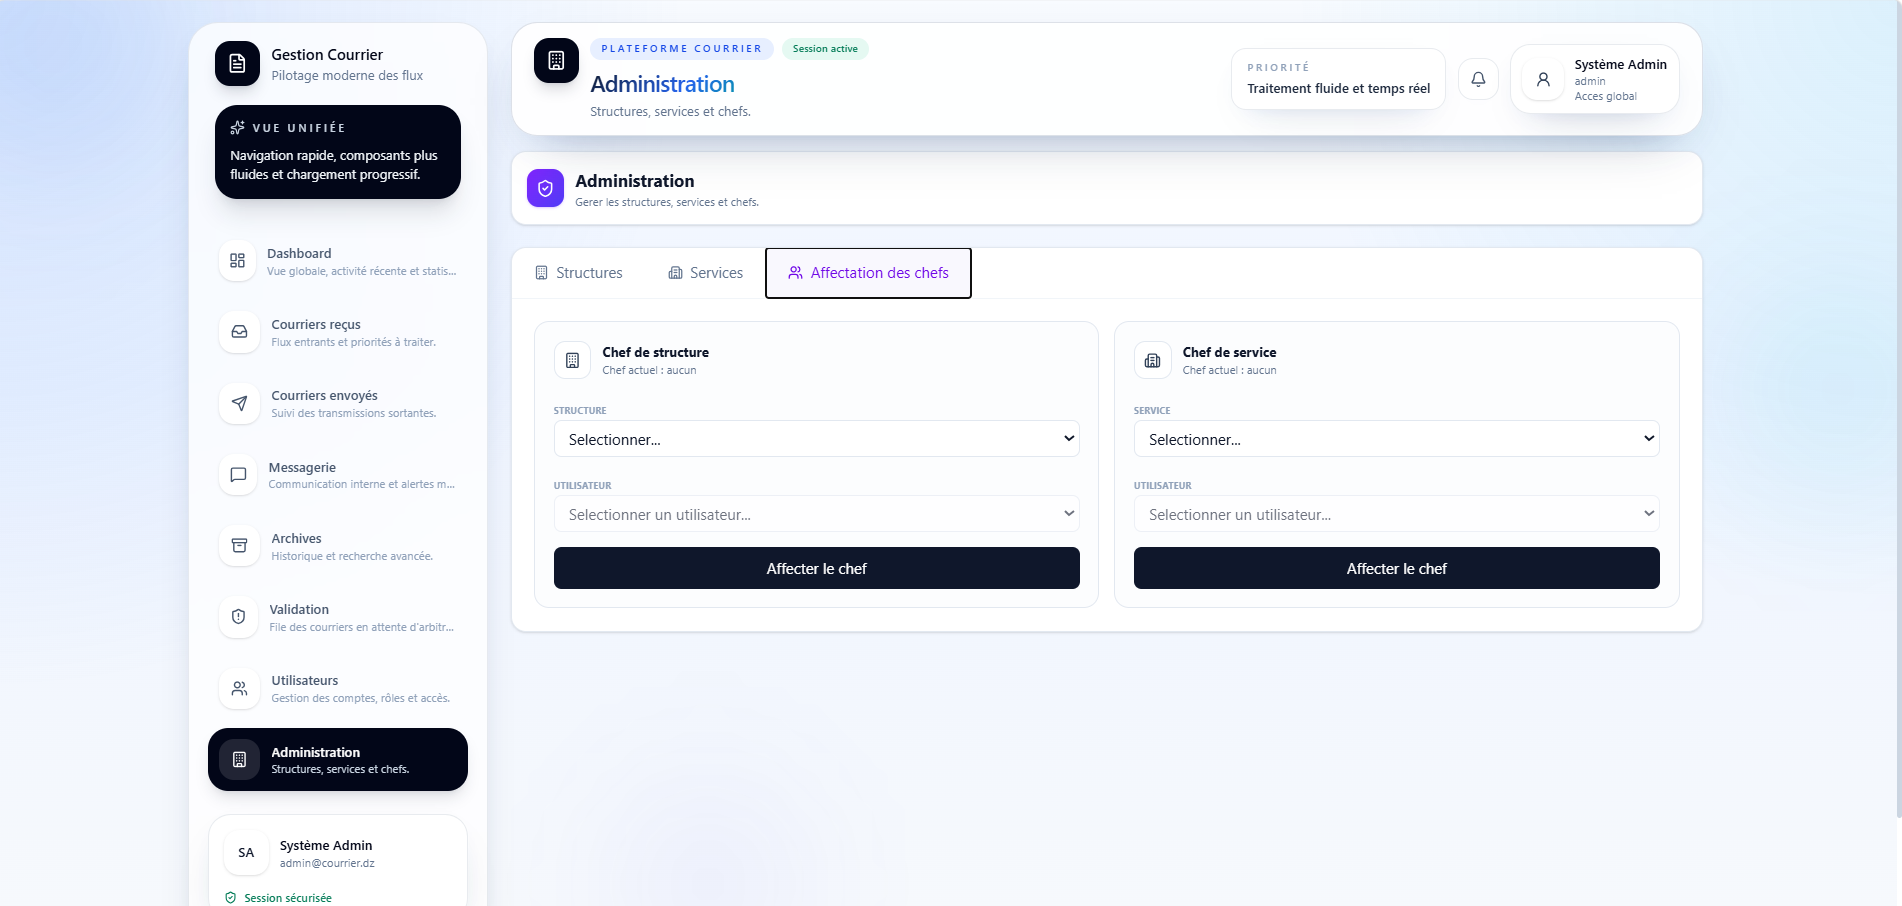
\includegraphics[width=0.88\textwidth,height=0.42\textheight,keepaspectratio]{images/app/affect.png}
    \caption{Affectation des responsables}
    \label{fig:affectation_responsables}
\end{figure}